%%%%%%%%%%%%%%%%%%%%%%%%%%%%%%%%%%%%%%%%%
% Template ini dibuat untuk makalah kolokium mahasiswa
% Program Alih Jenis (Ekstensi) Ilmu Komputer IPB
% Version 1.0 (18/05/2015)
%
% Template ini menggunakan template yang di-download dari:
% http://www.LaTeXTemplates.com
% Mathias Legrand (legrand.mathias@gmail.com)
% License: CC BY-NC-SA 3.0 (http://creativecommons.org/licenses/by-nc-sa/3.0/)
%
% Dimodifikasi untuk keperluan Program Studi
% Oleh: JULIO ADISANTOSO (julioipb@gmail.com)
%
% Untuk memudahkan penggunaan, maka diambil contoh makalah atas nama 
% Fithranto Faturakhman di bawah bimbingan Karlisa Priandana ILKOM-IPB.
% Silakan mengganti dan melengkapi file:
%    (1) kolokium_information.tex -- judul, nama, nim, email, pembimbing, dsb
%    (2) abstrak.tex -- abstrak makalah
%    (3) pendahuluan.tex -- berisi latar belakang, dsb
%    (4) metode.tex -- berisi metode penelitian
%    (5) pustaka.bib -- berisi daftar pustaka
%
%%%%%%%%%%%%%%%%%%%%%%%%%%%%%%%%%%%%%%%%%

%----------------------------------------------------------------------------------------
%	PACKAGES AND OTHER DOCUMENT CONFIGURATIONS
%----------------------------------------------------------------------------------------

\documentclass[fleqn,11pt]{SelfArx} % Document font size and equations flushed left
\usepackage[english]{babel}
\usepackage{adjustbox}

%----------------------------------------------------------------------------------------
%	COLUMNS
%----------------------------------------------------------------------------------------

\setlength{\columnsep}{0.55cm} % Distance between the two columns of text
\setlength{\fboxrule}{0.75pt} % Width of the border around the abstract

%----------------------------------------------------------------------------------------
%	COLORS
%----------------------------------------------------------------------------------------

\definecolor{color1}{RGB}{0,0,90} % Color of the article title and sections
\definecolor{color2}{RGB}{0,20,20} % Color of the boxes behind the abstract and headings

%----------------------------------------------------------------------------------------
%	HYPERLINKS
%----------------------------------------------------------------------------------------

\usepackage{hyperref} % Required for hyperlinks
\hypersetup{hidelinks,colorlinks,breaklinks=true,urlcolor=color2,citecolor=color1,linkcolor=color1,bookmarksopen=false,pdftitle={Title},pdfauthor={Author}}


%
% Hyphenation untuk Indonesia 
%
% @author  Andreas Febrian
% @version 1.00
% 
% Tambahkan cara pemenggalan kata-kata yang salah dipenggal secara otomatis 
% oleh LaTeX. Jika kata tersebut dapat dipenggal dengan benar, maka tidak 
% perlu ditambahkan dalam berkas ini. Tanda pemenggalan kata menggunakan 
% tanda '-'; contoh: menarik  --> pemenggalan: me-na-rik
%

\hyphenation{
    % alphabhet A
    a-na-li-sa a-tur 
    a-pli-ka-si 
    % alphabhet B
    ba-ngun-an 
    be-be-ra-pa 
    ber-ge-rak
    ber-ke-lan-jut-an 
    ber-pe-nga-ruh 
    Bha-dri-ra-ju
    % alphabhet C
    ca-ri
    % alphabhet D
    di-sim-pan di-pim-pin de-ngan da-e-rah di-ba-ngun da-pat di-nya-ta-kan 
    di-sim-bol-kan di-pi-lih di-li-hat de-fi-ni-si
    % alphabhet E
    e-ner-gi eks-klu-sif
    % alphabhet F
    fa-si-li-tas
    % alphabhet G
    ga-bung-an ge-rak
    % alphabhet H
    ha-lang-an
    % alphabhet I
    % alphabhet J
    jang-krik
    % alphabhet K
    ke-hi-lang-an
    ku-ning 
    kua-li-tas ka-me-ra ke-mung-kin-an ke-se-pa-ham-an
    % alphabhet L
    ling-kung-an
    % alphabhet M
    me-neng-ah
    meng-a-tas-i me-mung-kin-kan me-nge-na-i me-ngi-rim-kan 
    meng-u-bah meng-a-dap-ta-si me-nya-ta-kan mo-di-fi-ka-si
    meng-a-tur meng-um-pul-kan Men-te-ri
    Mo-ham-med
    % alphabhet N
    nya-ta non-eks-klu-sif
    % alphabhet O
    % alphabhet P
	pe-nye-rap-an 
	pe-ngon-trol
    pe-mo-del-an
    pe-ran  pe-ran-an-nya
    pem-ba-ngun-an pre-si-den pe-me-rin-tah prio-ri-tas peng-am-bil-an 
    peng-ga-bung-an pe-nga-was-an pe-ngem-bang-an 
    pe-nga-ruh pa-ra-lel-is-me per-hi-tung-an per-ma-sa-lah-an 
    pen-ca-ri-an peng-struk-tur-an
    PER-TAM-BANG-AN
    % alphabhet Q
    % alphabhet R
    ran-cang-an
    % alphabhet S
    si-mu-la-si sa-ngat Sa-ma-rin-da
    % alphabhet T
    te-ngah
    ter-da-pat
    % alphabhet U
    % alphabhet V
    % alphabhet W
    % alphabhet X
    % alphabhet Y
    % alphabhet Z
    % special
}
% Tuliskan nama lengkap Anda
\def\namaMhs {Jeannette Claudya Weya Pantouw}

% Tuliskan NIM Anda
\def\nim {G64144029}

% Tuliskan alamat email Anda
\def\emailMhs {jeanclaudyawp@gmail.com}

% Tuliskan nama lengkap dosen pembimbing
\def\namaDosen {Julio Adisantoso}

% Tuliskan judul makalah kolokium di definisi "judul"
\def\judul {Analisis Sentimen dengan Klasifikasi Rocchio pada Data Twitter Bahasa Indonesia}

% Tuliskan kata kunci, dipisahkan oleh tanda titik-koma
\def\katakunci {Analisis sentimen; Kementrian; Multinomial; Pendidikan; Rocchio}


\usepackage{xcolor,colortbl}
\usepackage{multicol}
\usepackage{multirow}
\usepackage{graphicx,xcolor}
\graphicspath{{gambar/}}

\usepackage[urldate=comp, backend=biber, style=authoryear, url=true, doi=true, maxbibnames=4, maxcitenames=2, block=none, sorting=nyt]{biblatex}
\usepackage{xpatch}
\addbibresource{pustaka.bib}
\DefineBibliographyStrings{english}{%
	and = {dan}
}
\DefineBibliographyStrings{english}{%
	andothers = {\em et\addabbrvspace al\adddot}
}
\renewbibmacro{in:}{
	\iffieldundef{journaltitle}
	{}
	{\xspace dalam:}
}
\renewbibmacro*{volume+number+eid}{%
	\printfield{volume}%
	%  \setunit*{\adddot}% DELETED
	\setunit*{\addnbspace}% NEW (optional); there's also \addnbthinspace
	\printfield{number}%
	\setunit{\addcomma\space}%
	\printfield{eid}}
\DeclareFieldFormat[article]{number}{\mkbibparens{#1}}
\DeclareFieldFormat{url}{\printtext{Dapat diunduh dari}\addcolon\space\url{#1}}
%\DeclareFieldFormat{urldate}{#1}
\DeclareFieldFormat{urldate}{%
	\thefield{urlday}\addslash%
	\thefield{urlmonth}\addslash%
	\thefield{urlyear}\isdot}

\renewbibmacro*{url+urldate}{%
	\iffieldundef{urlyear}
	{}
	{\setunit*{\addspace}%
		\printtext{[Internet]. [}%
		\printtext{Diunduh tanggal}\space%
		\printurldate\space
		\printtext{].}\space%
		\printfield{url}}%
}
\xpatchbibmacro{date+extrayear}{%
  \printtext[parens]%
}{%
  \setunit{\addperiod\space}%
  \printtext%
}{}{}
\nocite{*}


%\usepackage[urldate=iso8601, backend=biber, style=authoryear, url=true, doi=true, sorting=nyt]{biblatex}
%\addbibresource{pustaka.bib}
%\DefineBibliographyStrings{english}{%
%	urlseen = {diunduh pada},
%}
%\renewbibmacro{in:}{\xspace dalam:}
%\renewbibmacro*{volume+number+eid}{%
%	\printfield{volume}%
%	%  \setunit*{\adddot}% DELETED
%	\setunit*{\addnbspace}% NEW (optional); there's also \addnbthinspace
%	\printfield{number}%
%	\setunit{\addcomma\space}%
%	\printfield{eid}}
%\DeclareFieldFormat[article]{number}{\mkbibparens{#1}}

%----------------------------------------------------------------------------------------
%	ARTICLE INFORMATION
%----------------------------------------------------------------------------------------

\JournalInfo{Makalah Kolokium Program S1 Ilmu Komputer Alih Jenis} % Journal information
\Archive{Departemen Ilmu Komputer, FMIPA-IPB} % Departemen ILKOM-IPB

\PaperTitle{\judul} 

\Authors{\namaMhs (\nim)*, \namaDosen} % Penulis
\affiliation{*\scriptsize\textbf{Alamat Email}: \emailMhs \normalsize} % Corresponding author

\Keywords{\scriptsize \katakunci \normalsize} 
\newcommand{\keywordname}{Kata Kunci} % Defines the keywords heading name

%----------------------------------------------------------------------------------------
%	ABSTRACT
%----------------------------------------------------------------------------------------
\Abstract{\scriptsize 
	% ---- Tuliskan abstrak di bagian ini seperti contoh.
	Penelitian ini menganalisis sentimen masyarakat terhadap kementrian dan pendidikan di Indonesia. Untuk itu dalam pengumpulan data kata kunci “kementrian”, “pendidikan”, “sekolah”, dan “Indonesia” digunakan untuk menjaring data terkait isu ini. Penelitian ini melakukan klasifikasi orientasi sentimen dalam 3 jenis yaitu positif, negatif dan netral menggunakan. Penelitian analisis sentimen sebelumnya juga dilakukan oleh Adityawan (2014) mengenai klasifikasi \textit{Naïve Bayes} pada pesan twitter menggunakan data seimbang belum menunjukan akurasi yang cukup baik yaitu 66.42\% untuk model Multinomial dan 71.09\% untuk model Bernoulli. Untuk itu pada penelitian ini, akan dilakukan penelitian menggunakan metode yang berbeda, yaitu metode berbasis vektor untuk menganalisis apakah hasil klasifikasi metode berbasis vektor memiliki akurasi yang lebih baik dari berbasis peluang. Penelitian ini akan menganilisis hasil perbandingan antara metode klasifikasi konvensional yaitu \textit{Multinomial Naïve Bayes} dengan metode klasifikasi Rocchio. Metode Rocchio akan digunakan  untuk mengklasifikasikan data tweet, dengan menggunakan pendekatan berdasarkan kedekatan (\textit{similarity}) .
	% ---- Akhir bagian abstrak
	\normalsize}


%----------------------------------------------------------------------------------------

\begin{document}

\flushbottom % Makes all text pages the same height

\maketitle % Print the title and abstract box

\thispagestyle{empty} % Removes page numbering from the first page

%----------------------------------------------------------------------------------------
%	BAGIAN PENDAHULUAN
%----------------------------------------------------------------------------------------

%----------------------------------------------------------------------------------------
%	PENDAHULUAN
%----------------------------------------------------------------------------------------
\section*{PENDAHULUAN} % Sub Judul PENDAHULUAN
% Tuliskan isi Pendahuluan di bagian bawah ini. 
% Jika ingin menambahkan Sub-Sub Judul lainnya, silakan melihat contoh yang ada.
% Sub-sub Judul 
\subsection*{Latar Belakang}

Analisis sentimen adalah bidang ilmu yang menganalisis opini, penilaian serta sentimen terhadap suatu isu tertentu (\cite{LIU2012}). Analisis sentimen juga dapat digunakan sebagai penentuan keputusan terhadap suatu isu atau masalah. Opini – opini yang selanjutnya akan digunakan sebagai data untuk penentuan keputusan tehadap isu yang ada. Analisis sentimen juga memegang peranan pada pengolahan opini yang mengandung polaritas, yaitu memiliki nilai sentimen yang positif ataupun negatif (\cite{Novantirani2014}). Sosial media merupakan tempat yang memungkinkan semua orang untuk mengekspresikan opini mereka ke publik (\cite{LIU2012}). Menurut Semiocast, lembaga riset media sosial yang berpusat di Paris, Prancis, jumlah pemilik akun Twitter di Indonesia merupakan yang terbesar kelima di dunia, dan berada pada posisi ketiga negara yang paling aktif mengirim pesan Twitter (tweet) perhari (Tempo 2012). Banyaknya pengguna Twitter dan adanya kemudahan dalam penyampaian opini melalui media ini, maka data opini berupa tweet tersebut yang kemudian dapat menjadi peluang dan dapat dimanfaatkan sebagai bahan penilaian, tingkat kepuasan dan evaluasi (Novantirani, 2014). Hal ini mendorong beberapa instansi atau kelompok tertentu untuk mendapatkan suatu informasi terkait isu yang akan dianalisis. 

Opini masyarakat dari twitter inilah yang akan digunakan selanjutnya menjadi data penelitian ini. Data tweet yang kemudian akan diolah menjadi data yang mengandung sentimen. Penelitian ini melakukan analisis terhadap data tweet terkait isu mengenai kementrian dan pendidikan. Data tweet inilah yang akan digunakan sebagai bahan penelitian untuk penilaian, tingkat kepuasan serta evaluasi kinerja pemerintahan khususnya di bidang kementrian dan pendidikan. Isu inilah yang akan menjadi kata kunci pengambilan data yang akan diolah selanjutnya. Pada penelitian Institute for Development of Economics and Finance (Indef) pada tahun 2015, berhasil menjaring 12 juta tweet terkait pemerintahan dan 150 ribu diantaranya memiliki tema pembangunan (Tempo 2015). Banyaknya jumlah tweet terkait pemerintahan khususnya dibidang kementrian dan pendidikan inilah yang mendorong dilakukannya penelitian ini dengan menyertakan kata tersebut tersebut sebagai kata kunci dalam pengumpulan data. 


Untuk dapat mengetahui informasi, data tweet perlu diolah yang selanjutnya dilakukan klasifikasi untuk mengetahui apakah isu tersebut masuk ke dalam sentimen positif, negatif, atau netral. Proses klasifikasi ini dapat dilakukan dengan beberapa metode. Metode klasifikasi yang umumnya digunakan yaitu berbasis peluang dan berbasis vektor. Untuk klasifikasi berbasis peluang metode yang dapat digunakan diantaranya \textit{naïve bayes} dengan pemodelan \textit{bernauli} dan \textit{multivariant}. Sedangkan untuk klasifikasi berbasis vektor, metode yang dapat digunakan diantaranya \textit{Rocchio algorithm}, \textit{k-Nearest Neighbor}, \textit{Descision Tree}, \textit{Support Vector Machines}.

Penelitian analisis sentimen sebelumnya juga dilakukan oleh \citeauthor{ADITYAWAN2014} (\cite*{ADITYAWAN2014}) mengenai klasifikasi Naïve Bayes pada pesan twitter menggunakan data seimbang belum menunjukan akurasi yang cukup baik yaitu 66.42\% untuk model Multinomial dan 71.09\% untuk model Bernoulli. Untuk itu pada penelitian ini, akan dilakukan penelitian menggunakan metode yang berbeda, yaitu metode berbasis vektor untuk menganalisis apakah hasil klasifikasi metode berbasis vektor memiliki akurasi yang lebih baik dari berbasis peluang. 

Penelitian ini menggunakan metode klasifikasi Rocchio dengan pendekatan kesamaan (\textit{similarity}) dan menggunakan tiga kategori sentimen yaitu netral, postif, dan negatif. Metode ini yang kemudian akan digunakan apakah data tweet masuk ke dalam sentimen positif, negatif ,atau netral. Rocchio dengan pendekatan similarity yang digunakan  karena similarity menghitung berdasarkan kedekatan dokumen. Dari sinilah selanjutnya dapat diperoleh kesimpulan data tweet yang ada terkait isu mengenai kementrian dan pendidikan mendapatkan sentimen seperti apa di kalangan masyarakat. 


% Sub-sub Judul 
\subsection*{Rumusan Masalah}
Berdasarkan latar belakang, perumusan masalah dalam penelitian ini adalah: 
\begin{enumerate}[noitemsep] 
	\item Bagaimana mengimplementasikan metode Rocchio pada analisis sentimen Twitter berbahasa Indonesia?
	\item Bagaimana perbandingan akurasi metode Rocchio dengan Multinomial Naïve Bayes ?

\end{enumerate}

\subsection*{Tujuan}
Tujuan penelitian ini adalah: 
\begin{enumerate}[noitemsep] 
	\item Mengimplementasikan analisis sentimen dengan menggunakan metode Rocchio pada data Twitter berbahasa Indonesia
	\item Membandingkan akurasi antara hasil klasifikasi analisis sentimen menggunakan metode Multinomial Naïve Bayes dengan metode Rocchio
	
\end{enumerate}

\subsection*{Manfaat}
Penelitian ini diharapkan dapat membantu entitas yang ingin mengetahui isu tertentu dari data Twitter. Penelitian ini juga diharapkan dapat memberikan informasi apakah isu tersebut mengandung sentiment positif, negative, atau netral.

\subsection*{Ruang Lingkup}
Tujuan penelitian ini adalah: 
\begin{enumerate}[noitemsep] 
	\item Penelitian ini menggunakan data Twitter tentang kementrian dan pendidikan di Indonesia.
	\item Pemilihan fitur menggunakan \textit{Inverse Document Frequency} (IDF).
	\item Membandingkan klasifikasi \textit{Multinomial Naive Bayes} dan \textit{Rocchio}
\end{enumerate}

%----------------------------------------------------------------------------------------
%	BAGIAN METODE
%----------------------------------------------------------------------------------------

%----------------------------------------------------------------------------------------
%	METODE
%----------------------------------------------------------------------------------------

\section*{METODE PENELITIAN}

Penelitian ini diawal dengan pengumpulan data selanjutnya masuk tahap ke indexing, kemudian membagi data tersebut menjadi data latih dan data uji. Data latih kemudian akan di klasifikasikan menggunakan metode klasifikasi Rocchio. Tahapan terakhir yaitu mengevaluasi hasil klasifikasi metode rochhio dengan data uji. Skema tahapan analisis sentimen dapat dilihat pada Gambar \ref{fig:tahapan} 

\begin{figure}[h!] % Gunakan \begin{figure*} untuk memasukkan Gambar
	\centering
	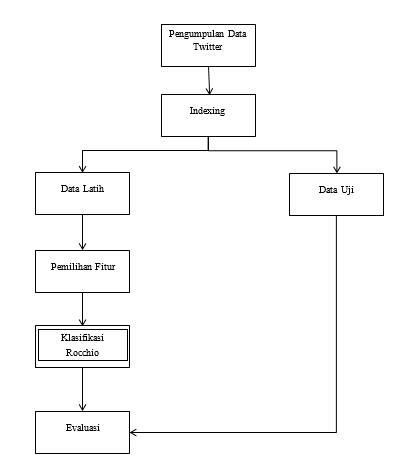
\includegraphics[width=200pt]{langkahkerja.png}
	\caption{Tahapan Penelitian Metode Klasifikasi Rocchio pada Sentimen Analisis Data Twitter}
	\label{fig:tahapan}
\end{figure}

\subsection*{Pengumpulan Data}
Tahapan dalam penelitian analisis sentimen ini yaitu diawali dengan pengumpulan data twitter. Data yang digunakan merupakan data \textit{post user}. \textit{Post} atau pesan dalam twitter dikenal dengan sebutan tweet (Zhang et al. 2011). Data yang akan diambil dari twitter adalah data dengan kata kunci “Kementrian” ,”mentri”, “Pendidikan”, “Sekolah”, dan “Indonesia”. Kata kunci tersebut digunakan  untuk mengambil data terkait opini – opini masyarakat di bidang kementrian dan pendidikan. Pada tahap akuisisi data tweet, data diperoleh dari tags.hawksey.info. Data yang didapatkan berupa data excel dengan atribut seperti yang terlihat pada Tabel \ref{tab:strukturdatatwitter}.

\begin{table}[hbt]
	\caption{Struktur Data Response Twitter}
	\centering
	\begin{tabular}{llr}
		
		\cmidrule(r){1-2}
		Atribut & Keterangan \\
		\midrule
		id\_str & id dari \textit{post} twitter \\
		from\_user & \textit{username} pemakai twitter \\
		text & \textit{post} twitter \\
		created\_at & tanggal dan waktu \textit{post} dibuat \\
		geo\_coordinates & koordinat tempat \textit{user} \\
		source & tautan profil \textit{user} \\
		profile\_image\_url & gambar profil dari \textit{user} \\
		user\_followers\_count & jumlah \textit{follower user} \\
		user\_friends\_count & jumlah teman \textit{user} \\
		user\_location & lokasi dari \textit{user} \\
		status\_url & link dari \textit{post} twitter \\
		
		\bottomrule
	\end{tabular}
	\label{tab:strukturdatatwitter}
\end{table}

Tabel \ref{tab:strukturdatatwitter} merupakan informasi struktur data Twitter yang diperoleh dari tags.hawksey.info. Data yang diperoleh dari sistem masih berupa data mentah post user yang belum ada sentimennya. Data dengan atribut text yang akan diambil untuk diproses selanjutnya. Data atribut text ini yang selanjutnya akan diolah sentimennya. Proses pengolahan data mentah menjadi sentimen dilakukan secara manual. Jumlah data yang digunakan pada penelitian ini sebanyak 6000 data yang sudah diberi sentimen. Dari data tersebut akan dibagi menjadi dua, yaitu data latih sebanyak 70\% dan data uji sebanyak 30\%. 


\subsection*{Indexing}

Setelah data didapatkan dan memiliki sentimen tahap selanjutnya yaitu \textit{indexing}. \textit{Indexing} merupakan proses persiapan yang dilakukan terhadap dokumen sehingga dokumen siap untuk diproses. Proses \textit{indexing} dibagi menjadi dua proses, yaitu \textit{document indexing} dan \textit{term indexing}. Dari \textit{term indexing} akan dihasilkan koleksi kata yang akan digunakan untuk meningkatkan performansi pencarian pada tahap selanjutnya. Selain itu, teknik \textit{indexing} ini juga dilakukan agar hasil yang diperoleh lebih baik. Karena kebanyakan \textit{tweet} hanya berisi tautan dan tidak menunjukkan sentimen tertentu, dan penulisannya ditulis dalam bahasa asing (Parikh dan Movassate 2014). Bahasa asing yang dimaksud dalam penelitian adalah kata – kata yang dalam penulisannya menggunakan pengabungan antara alfanumerik dan simbol – simbol lainnya. Ada beberapa tahapan  yang dilakukan didalam proses \textit{indexing} diantaranya \textit{tokenizing}, pengahapusan \textit{stopwords}, normalisasi kata, \textit{stemming}, dan pembuatan \textit{document term matrix}.


\subsection*{Tokenizing}
Tahap awal dalam proses \textit{indexing} adalah \textit{tokenizing}. Pada tahap ini setiap data \textit{post twitter} yang berupa kata – kata akan diubah menjadi kumpulan term, dengan tidak menyertakan mention, URL, tanda baca, dan angka pada \textit{tweet}. Selain itu, semua data pada tweet juga akan diubah menjadi huruf kecil. Proses memotong dokumen atau kata menjadi bagian-bagian yang lebih kecil disebut token. Token bisa berupa paragraf, kalimat, frasa kata tunggal sederhana, dan konsep. Teknik yang digunakan dalam proses tokenisasi adalah segmentasi dan memilah. Sebagai contoh, jika ada masukkan teks “Pendidikan di Indonesia sangat buruk dan sungguh memprihatinkan”, maka hasil keluaran dari proses \textit{tokenizing} adalah seperti yang disajikan pada Tabel \ref{tab:tokenizing}.

\begin{table}[hbt]
	\caption{Tokenizing}
	\centering
	\begin{tabular}{llr}
		\toprule
		Input & \multicolumn{2}{c}{Data Twitter} \\
		\midrule
		Output & Data & Twitter \\
		\bottomrule
	\end{tabular}
	\label{tab:tokenizing}
\end{table}

Tabel \ref{tab:tokenizing} merupakan contoh hasil proses \textit{tokenizing}, setiap kalimat yang ada akan dipilah menjadi potongan – potongan kata. Pada penelitian ini \textit{tokenizing} dilakukan dengan menggunakan kode dari Nette yang didapat dari https://github.com/nette/tokenizer.


\subsection*{Penghapusan Stopwords}

\textit{Stopwords} merupakan kata – kata atau term yang tidak berhubungan dan tidak memiliki makna atau informasi yang berhubungan dengan dokumen, walaupun kata tersebut sering muncul pada dokumen. \textit{Stopwords} adalah sebuah kata-kata dalam bahasa tertentu yang sangat umum digunakan dan memiliki nilai informasi nol (Meyer et.al . 2008). Penghapusan kata tersebut tidak akan mengubah makna dan isi dari informasi tweet, beberapa contoh stopwords dalam bahasa  Indonesia diantaranya: yang, juga, dari, dia, kami, kamu, aku, saya, ini, dan itu. Pada penelitian ini digunakan dataset daftar \textit{stopword} yang  didapatkan dari penelitian Tala (2003) sebanyak 759 kata. Dataset penelitian Tala inilah yang nantinya akan digunakan untuk menghapus \textit{stopword} pada data \textit{tweet}.


\subsection*{Normalisasi Kata}

Normalisasi kata merupakan proses penggantian kata yang tidak baku menjadi kata baku. Normalisasi ini dilakukan untuk mempermudah proses penelitian pada tahapan selanjutnya. Kata baku akan cenderung lebih kecil ambiguitas dibandingkan dengan kata yang tidak baku, untuk itu normalisasi dilakukan untuk mentranslasi kata tidak baku menjadi baku (Aziz 2013). Untuk itu perlu dilakukan normalisasi kata dengan cara mengganti kata yang tidak baku (Sproat et al. 2001). Pada penelitian ini proses pengantian kata tidak baku menjadi baku menggunakan dataset yang sudah ada. Dataset yang digunakan adalah sebuah kamus yang berisi kumpulan data tidak baku dengan kata bakunya. Hal ini dilakukan untuk memudahkan proses penggantian kata. Dataset kata tidak baku dan kata baku yang digunakan sebanyak 3719 baris data. 

\subsection*{Stemming}

\textit{Stemming} merupakan proses transformasi kata – kata menjadi kata dasarnya dalam sebuah teks dokumen, hal ini juga digunakan untuk meningkatkan performa IR (Agusta, 2009). \textit{Stemming} adalah  proses  konversi term ke  bentuk  umumnya. Tidak hanya ditransformasi menjadi kata dasar, tetapi kata – kata juga dapat ditransformasikan ke dalam bentuk sinonim kata tersebut. Sinonim adalah kata yang memiliki kesamaan makna tetapi berbeda dari sudut pandang morfologis. Contoh stemming dapat dilihat pada gambar \ref{fig:steming} 

\begin{figure}[h!] % Gunakan \begin{figure*} untuk memasukkan Gambar
	\centering
	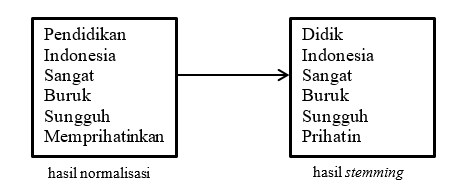
\includegraphics[width=200pt]{steming.png}
	\caption{Stemming}
	\label{fig:steming}
\end{figure}

Tahap \textit{stemming} bertujuan untuk mengurangi jumlah kata dan mendapatkan kata dasar yang benar-benar sesuai. Untuk itu penghapusan kata dan berbagai variasi lainnya seperti \textit{prefix} dan \textit{suffix} perlu dilakukan. Penelitian ini menggunakan algoritma Nazief dan Adriani (1996) dan kamus kata dasar  yang digunakan sebanyak 28.526 kata.

\subsection*{Pembuatan Document Term Matrix (DTM)}

\textit{Term Document Matrix} (TDM) dilakukan untuk menghitung jumlah kemunculan kata pada dokumen (Nadilah 2016). Cara yang paling umum untuk merepresentasikan teks ke dalam bentuk matrik adalah melalui pembuatan DTM. DTM dapat diekspor dari korpus dan digunakan sebagai mekanisme \textit{bag-of-words}. Pendekatan ini menghasilkan matrik dengan id dokumen sebagai baris dan \textit{term} sebagai kolom. Setiap elemen matrik yang ada merupakan representasi dari frekuensi kemunculan kata.
Sebagai contoh ada dua dokumen dengan id 1 dan 2 mempunyai kata yang sama yaitu “Saya suka makan nasi dan saya suka ayam goreng” dan “ayam goreng”. Tabel \ref{tab:dtm} menunjukkan contoh DTM yang terbentuk.
.

\begin{table}[hbt]
	\caption{Document Term Matrix}
	\centering
	\begin{adjustbox}{max width=\textwidth}
		\begin{tabular}{*{7}{c}}%%{llr}
			\toprule
			ID & saya & suka & makan & nasi & dan & ayam \\
			\midrule
			1 & 2 & 2 & 1 & 1 & 1 & 1 \\
			2 & 0 & 0 & 0 & 0 & 1 & 1 \\
			\bottomrule
		\end{tabular}
	\end{adjustbox}
	\label{tab:dtm}
\end{table}

Sedangkan pada penelitian ini, kolom matriks menunjukkan kata yang ada pada data \textit{tweet}, dan baris matriks menunjukkan indeks dari dokumen pada kumpulan korpus. Pada penelitian ini satu tweet menandakan satu dokumen.

\subsection*{Pembagian Data}

Data yang dihasilkan setelah proses \textit{indexing} dibagi  menjadi  dua subset data yaitu data latih dan data uji dengan perbandingan 70:30. Sebanyak 70 persen data latih dan 30 persen data uji. Data latih ini akan digunakan untuk tahapan selanjutnya sementara data uji digunakan untuk melakukan pengujian terhadap sistem klasifikasi yang telah dibuat dalam penelitian ini.

\subsection*{Pemilihan Fitur}

Pemilihan fitur merupakan proses pemilihan term yang mewakili informasi penting dari suatu dokumen atau teks. Adanya pemilihan fitur ini dapat meningkatkan akurasi karena adanya seleksi pada \textit{term} yang bukan merupakan penciri (Manning et all. 2008). Menurut Garnes (2009) pemilihan fitur secara umum dibagi menjadi dua metode, yaitu \textit{unsupervised feature selection} dan \textit{supervised feature selection}. Metode \textit{Unsupervised feature selection} tidak menggunakan informasi kelas dalam data latih ketika memilih fitur untuk \textit{classifier}, contohnya adalah \textit{Inverse Document Frequency} (IDF). Sedangkan \textit{Supervised feature selection}  adalah metode seleksi fitur yang menggunakan informasi kelas dalam data latih, sehingga \textit{set pre-classied} harus tersedia agar seleksi fitur dapat dilakukan. Pada penelitian ini pemilihan fitur yang akan digunaka yaitu IDF. IDF dipilih karena metode ini efisien, mudah dan memiliki hasil yang akurat (Robertson 2005).


\subsection*{Inverse document frequency (IDF)}

\textit{Inverse Document Frequency} (IDF) merupakan salah satu metode yang digunakan dalam pemilihan fiitur.  Sebelum masuk ke tahapan klasifikasi, pembobotan dilakukan pada setiap data yang ada untuk dapat menghitung kesamaan dan jarak antar data traning dengan data uji. Pada Penelitian ini untuk menghitung bobot setiap kata dalam dokumen digunakan skema pembobotan IDF. \newline 
\textit{Inverse document frequency} (IDF) adalah \textit{inverse} atau kebalikan dari nilai DF. Hal ini dikarenakan \textit{term} yang sering muncul di dokumen dianggap sebagai term umum, sehingga tidak penting nilainya, sehingga ukuran kepentingan suatu term dari dokumen yang akan digunakan penciri yang memiliki nilai kecil dengan rentang yang tidak begitu jauh. Sebaliknya \textit{term} yang jarang muncul pada dokumen perlu diperhatikan dalam pembobotan. Menurut Witten (1999) kata yang jarang atau paling sedikit muncul justru harus diperhatikan sebagai kata yang lebih penting dari pada kata yang paling sering muncul dalam dokumen. Banyaknya dokumen d yang mengandung \textit{term} t tertentu disebut DF. Ukuran kepentingan suatu term dari dokumen yang digunakan sebagai penciri adalah nilai DF yang besar, namun nilai dari DF memiliki rentang nilai yang lebar. Nilai IDF dapat diperoleh dari persamaan [\ref{eq:persamaanidf}]

\begin{equation}
idf\textsubscript{t} = log(\frac{N}{df\textsubscript{t}})
\end{equation}

Pada persamaan \ref{eq:persamaanidf} variabel N adalah banyaknya dokumen dan sedangkan df adalah banyaknya dokumen didalam koleksi yang mengandung \textit{term} tertentu, sehingga dapat dikatakan bahwa IDF merupakan frekuensi \textit{term} atau data yang jarang muncul dalam suatu dokumen.

\subsection*{Mutual information (MI)}

\textit{Mutual information} (MI) merupakan seleksi fitur yang melibatkan kontribusi term. MI mengukur seberapa besar kontribusi keberadaan suatu \textit{term} t,dalam pembuatan keputusan klasifikasi yang benar. MI juga menunjukan keputusan klasifikasi secara benar atau salah melalui kontribusi keberadaan term tersebut. Nilai dari MI disimbolkan dengan notasi I, dimana [\ref{eq:persamaanmi}]

\begin{equation}
\begin{split}
\tiny
I(U;C) = \sum\limits_{et\in\{1,0\}}\sum\limits_{ec\in\{1.0\}} P(U = et, C = ec) \\
log_2 \frac{P(U = et,C =ec)}{P(U = et)P(C = ec)} 
\label{eq:persamaanmi}
\normalsize
\end{split}
\end{equation}

Pada persamaan (2) U adalah variabel acak dengan nilai-nilai et = 1 , yang menunjukkan bahwa dokumen berisi term t, sedangkan untuk et = 0 menunjukkan bahwa dokumen tidak mengandung t, dan C adalah variabel acak dengan nilai-nilai ec = 1 (dokumen di kelas c) dan ec = 0 (dokumen tidak di kelas c). Nilai dari I juga bisa dijabarkan menjadi persamaan berikut : [\ref{eq:persamaanmilanjut}]

\begin{equation}
\begin{split}
\tiny
\frac{N_{11}}{N}log_2\frac{NN_{11}}{N_1N_1} + \frac{N_{01}}{N}log_2\frac{NN_{01}}{N_0N_1} + \\
\frac{N_{10}}{N}log_2\frac{NN_{11}}{N_1N_0} + \frac{N_{00}}{N}log_2\frac{NN_{00}}{N_0N_0}
\label{eq:persamaanmilanjut}
\normalsize
\end{split}
\end{equation}

Pada persamaan (3) nilai N adalah jumlah dokumen yang memiliki nilai-nilai et dan ec yang ditunjukan oleh dua \textit{subscript}. Sebagai contoh, N10 adalah jumlah dokumen yang mengandung \textit{term} t (et = 1) dan tidak dalam c (ec = 0). N1. = N10 + N11 adalah jumlah dokumen yang berisi \textit{term} t (et = 1) dan untuk menghitung dokumen independen keanggotaan kelas (ec $\in$ {0, 1}). N adalah jumlah total dokumen atau N= N00 + N01 + N10 + N11. 

\subsection*{Chi-Square (X\textsuperscript{2})}
\textit{Chi-square}  (x\textsuperscript{2})adalah suatu ukuran yang menyatakan perbedaan antara frekuensi observasi (O) dan frekuensi harapan (E) untuk setiap term (i) yang dirumuskan dengan persamaan: [\ref{eq:chi}]

\begin{equation}
\begin{split}
\tiny
X^2(D, t, c) = \sum\limits_{et\in\{1,0\}}\sum\limits_{et\in\{1,0\}} \frac{(N_{etec} - E_{etec})^2}{E_{etec}}
\label{eq:chi}
\normalsize
\end{split}
\end{equation}

Sedangkan D adalah variabel acak dengan nilai-nilai et = 1 adalah dokumen berisi term t dan et = 0 adalah dokumen yang tidak mengandung t, ec = 1 adalah dokumen di kelas c dan ec = 0 adalah dokumen tidak di kelas c. N adalah frekuensi yang diamati dalam dokumen D dan E adalah frekuensi yang diharapkan. Pengambilan keputusan dilakukan berdasarkan nilai dari masing-masing kata. Kata yang memiliki nilai X2 di atas nilai kritis pada taraf nyata adalah kata yang akan dipilih sebagai penciri dokumen. Kata yang dipilih sebagai penciri merupakan kata yang memiliki pengaruh terhadap kelas c. Nilai kritis  X2  untuk taraf nyata $\alpha$ yang digunakan dalam penelitian ini ditunjukkan pada Tabel  \ref{tab:chisquare}.

\begin{table}[hbt]
	\caption{Nilai kritis untuk taraf nyata $\alpha$}
	\centering
	\begin{tabular}{llr}
		\toprule
		$\alpha$ & Nilai Kritis \\
		\midrule
		0.050 & 3.840 \\
		0.010 & 6.630 \\
		0.005 & 7.880 \\
		\bottomrule
	\end{tabular}
	\label{tab:chisquare}
\end{table}

Pada penelitian ini akan menggunakan IDF sebagai seleksi fiturnya. IDF dipilih karena metode ini efisien, mudah dan memiliki hasil yang akurat Robertson (2005).

\subsection*{Klasifikasi}
Pada analisis sentimen klasifikasi digunakan untuk mengkategorikan setiap data yang ada ke kelas pencirinya. Salah satu tujuan dari klasifikasi teks atau dokumen adalah penggolongkan atau mengelompokkan suatu dokumen ke dalam suatu kategori tertentu
(Manning et all. 2008). Klasifikasi juga bertujuan untuk memprediksi karakteristik dari suatu objek. Klasifikasi juga dapat digunakan untuk mendeteksi sentimen terhadap suatu isu. Data hasil indexing akan diklasifikasikan terhadap analisis sentiment. Pada penelitian ini terdiri 3 kelas sentimen yang digunakan, yaitu positif, negatif, dan netral. Fungsi klasifikasi secara umum untuk memetakan suatu dokumen ke dalam kategori tertentu yaitu :

[\ref{eq:klasifikasi}]

\begin{equation}
\begin{split}
\tiny
\gamma : X -> C
\label{eq:klasifikasi}
\normalsize
\end{split}
\end{equation}
Secara umum fungsi ini yang akan dipakai untuk mengelompok data ke dalam himpunan kelas atau kategori yang ada, dengan X adalah kumpulan dokumen dan C merupakan kategori. Fungsi klasifikasi terbagi menjadi dua metode yaitu, berbasis vektor dan berbasis peluang (Manning et all. 2009). Secara garis besar pada pendekataan berbasis peluang, penentuan kelas pada sebuah dokumen atau data adalah dengan cara menghitung peluang keberadaan data tersebut dalam suatu kelas. Metode yang sering digunakan adalah metode \textit{Naïve Bayes}. Sedangkan pada pendekatan berbasis vektor, penentuan kelas pada sebuah data dilakukan dengan cara menghitung jarak data tersebut ke centroid suatu kelas. Metode yang sering digunakan pada pendekatan ini adalah metode Rocchio dan k Nearest Neighbor (KNN).

\subsection*{Metode Naive Bayes}
Model klasifikasi Multinomial dan Bernoulli merupakan metode klasifikasi berbasis peluang yang paling sering digunakan. Model klasifikasi ini banyak digunakan karena mudah diaplikasikan dan prosesnya sederhana (Manning et al. 2008). Pada model Multinomial Bernoulli  setiap dokumen memiliki atribut yang menunjukkan ada atau tidaknya kata- kata atau \textit{term} dalam dokumen tersebut, tetapi jumlah kemunculan term dalam dokumen tidak ikut diperhitungkan. Pada model Multinomial \textit{Naïve Bayes}, jumlah kemunculan term pada dokumen ikut diperhitungkan, setiap dokumen diwakili oleh kemunculan \textit{term} dari dokumen. Pada model ini, dapat diasumsikan jika kemunculan masing-masing term t bersifat independen antara satu term dengan yang lainnya. Dengan menggunakan nilai dari P(c/d) peluang suatu dokumen d di dalam kelas c dapat ditulis sebagai (Manning et al. 2009) [\ref{eq:multinb}]

\begin{equation}
\begin{split}
P(C|d) \alpha P(c) \Xi_{1\le k\le nd}P(t_k|c)
\label{eq:multinb}
\end{split}
\end{equation}

dengan P(tk|c) adalah peluang dari suatu term tk muncul pada dokumen d yang diketahui memiliki kelas c. Pendugaan parameter P (tk|c) dihitung dengan cara: [\ref{eq:multinblanjut}]

\begin{equation}
\begin{split}
\tiny
P(t_k|C) = \frac{T_{ct}}{\sum _{t' \in V} T_{ct'}}
\label{eq:multinblanjut}
\normalsize
\end{split}
\end{equation}

dengan Tct adalah jumlah kemunculan term t dalam dokumen training yang berada di kelas c.  adalah jumlah seluruh term yang muncul berulang kali pada dokumen yang sama (Manning et al. 2009).
\textit{Term} tidak selalu muncul pada salah satu kelas saat dilakukan klasifikasi sehinggga nilai p (tk |c) yang dihasilkan adalah nol. Untuk mengatasi permasalahan tersebut, digunakan laplace smoothing, yaitu menambahkan frekuensi term sebanyak 1 sehingga perhitungan dari p (tk |c)  menjadi (Manning et al. 2009)    
[\ref{eq:multinblanjutb}]

\begin{equation}
\begin{split}
\tiny
P(t_k|C) = \frac{T_{ct}}{\sum _{t' \in V} T_{ct'} + B}
\label{eq:multinblanjutb}
\normalsize
\end{split}
\end{equation}

\subsection*{Metode Rocchio}
Klasifikasi ini merupakan salah satu metode pembelajaran \textit{supervised document classification}. Metode \textit{Rocchio relevance feedback} adalah strategi reformulasi query paling populer karena sering digunakan untuk membantu user pemula suatu \textit{information retrieval systems} (Joachims 2013). Dalam siklus \textit{relevance feedback}, kepada user disajikan hasil pencarian dokumen, setelah itu user dapat memeriksa dan menandai dokumen yang benar-benar relevan Klasifikasi yang digunakan pada penelitian ini adalah fungsi klasifikasi dengan basis vektor, yaitu metode klasifikasi Rocchio. Klasifikasi rocchio merepresentasikan data ke dalam sebuah vektor. Kedekatan kesamaan isi dihitung dari kedekatan sudut yang terbentuk antara bobot data training dan bobot data test menggunakan aturan sodinus. Untuk menghitung bobot setiap kata dalam dokumen digunakan skema pembobotan TFIDF (Term Frequency / Invers Document Frequency) karena komponen heuristic utama adalah dalam klasifikasi rocchio yaitu skema pembobtan tfidf, untuk itu metode pembelajaran rocchio disebut juga dengan TFIDF Classifiers (Joachihms 1997). Pendekatan ini menggunakan perhitungan jarak atau kemiripan suatu data dengan pusat sebuah kelas. Metode ini membagi ruang vektor menjadi beberapa bagian berdasarkan centroid yang ada. 

Pada penelitian ini setiap dokumen training direpresentasikan sebagai vektor. Setiap titik atau vektor dokumen traning akan diberikan label sesuai dengan kategori kelasnya. Contohnya saja seperti pada gambar \ref{fig:rocio} 

\begin{figure}[h!] % Gunakan \begin{figure*} untuk memasukkan Gambar
	\centering
	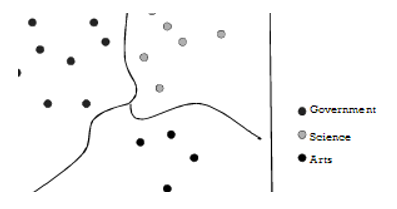
\includegraphics[width=200pt]{rocio.png}
	\caption{Pelabelan pada kategori kelas}
	\label{fig:rocio}
\end{figure}

Teknik Rocchio menerapkan batas - batas tersebut dalam bentuk\textit{ centroid} untuk memberi batasan tersebut. Nilai \textit{centroid} ini didapat dengan menghitung rata- rata jarak pada setiap data atau dokumen. \textit{Centroid} dapat diperoleh dari persamaan berikut [\ref{eq:rociosatu}]

\begin{equation}
\begin{split}
\mu (c) = \frac{1}{D_{c}} \sum \limits_{d\in D_c} v(d)
\label{eq:rociosatu}
\end{split}
\end{equation}

Kemudian selanjutnya dari masing masing vektor dokumen akan dicari nilai centroidnya dari setiap kelas yang ada menggunakan persamaan (10). Persamaan diatas digunakan untuk menghitung centroid dari kelas C, dimana Dc merupakan kumpulan dari dokumen di dalam korpus c, sedangkan v(d)merupakan vektor dokumen yang telah dinormalisasi. Terdapat dua cara untuk menentukan kemiripan dua vektor space model yaitu dengan mengukur jarak atau mengukur kemiripan. Untuk menentukan jarak kedekatan data uji ke dalam suatu kelas adalah dengan menghitung jarak antara kedua vektor menggunakan persamaan \textit{Euclidean}, yang didefinisikan sebagai berikut [\ref{eq:rociodua}]

\begin{equation}
\begin{split}
|x - y | = \sqrt{\sum_{i=1}^{m}(x_i - y_i)^2}
\label{eq:rociodua}
\end{split}
\end{equation}

Sedangkan untuk menghitung kemiripan antara dua vektor dokumen, didefinisikan dengan persamaan berikut [\ref{eq:rociotiga}]

\begin{equation}
\begin{split}
sim(d_1, d_2) = \frac{v(d_1).v(d_2)}{|v(d_1)||v(d_2)|}
\label{eq:rociotiga}
\end{split}
\end{equation}

Pada penelitian ini pendekatan yang akan digunakan untuk mencari kemiripan antara dua vector adalah pendekatan \textit{similarity}, sedangkan untuk pembobotannya digunakan IDF. Pendekatan ini digunakan karena pendekatan \textit{similarity} mencari kemiripan berdasarkan kesamaan, bukan berdasarkan kedekatan. Sedangkan pada pendekatan jarak, pengukuran dilakukan berdasarkan kedekatan. Kedekatan belum tentu menunjukkan kesamaan antar \textit{term}. Untuk itulah pendekatan menggunakan \textit{similarity} yang akan digunakan, yang selanjutnya diharapkan resiko kesalahan dalam pengambilan dokumen akan lebih sedikit terjadi.

\subsection*{Evaluasi}
Tahapan evaluasi adalah tahapan untuk mengetahui tingkat akurasi dan kinerja dari hasil klasifikasi menggunakan metode Rocchio. Kinerja klasifikasi dievaluasi dengan cara menghitung nilai akurasi, \textit{recall}, \textit{precision}, dan \textit{F-measure} dengan bantuan tabel \textit{confusion matrix}. \textit{Token} dari hasil seleksi fitur, akan dihitung peluangnya berdasarkan kelas-kelasnya dari dokumen Twitter. Setelah itu, membandingkannya dengan kelas aktual dari data uji dan kelas hasil prediksi dengan menggunakan \textit{confusion matrix}.
Menurut Manning (2008) terdapat dua parameter yang umum digunakan untuk mengukur kinerja sebuah sistem temu kembali informasi, yaitu \textit{precision} dan \textit{recall} Pengukuran efektivitas dilakukan untuk mengevaluasi system IR. Perlu adanya suatu tolak ukur yang digunakan untuk mengukur kualitas hasil klasifikasi. Pengukuran selanjutnya akan mengunakan nilai precision, recall, akurasi, dan F1. 

\subsection*{Precision}
\textit{Precision} adalah jumlah kelompok dokumen relevan dari total jumlah dokumen yang  ditemukan oleh sistem. \textit{Precision} direpresentasikan sebagai presentase dokumen yang di-retrieve yang benar-benar relevan. [\ref{eq:precision}]

\begin{equation}
\begin{split}
Precision = \frac{\#(relevant items retrieved)}{\#(retrieved items)} \\ 
= P(relevant|retrieved)
\label{eq:precision}
\end{split}
\end{equation}

\subsection*{Recall}
\textit{Recall} adalah rasio jumlah dokumen relevan yang ditemukan kembali dengan total jumlah dokumen dalam kumpulan dokumen yang dianggap relevan. [\ref{eq:recall}]

\begin{equation}
\begin{split}
Recall = \frac{\#(relevant items retrieved)}{\#(relevant items)} \\ 
= P(retrieved|relevant)
\label{eq:recall}
\end{split}
\end{equation}


\begin{equation}
\begin{split}
\tiny
P = tp/(tp+fp) \\ 
R = tp/(tp+fn)
\label{eq:evaluasi}
\normalsize
\end{split}
\end{equation}

\subsection*{Accuracy}
Setelah nilai precision dan recall didapatkan keakuratan hasil klasifikasi juga dinilai dari akurasinya, kemudian membandingkannya dengan kelas aktual dari data uji dan kelas hasil prediksi dengan menggunakan confusion matrix untuk untuk menghitung akurasi digunakan rumus seperti berikut dan mengacu tabel confusion matrix pada Table \ref{tab:konsep}. 

\begin{table}[hbt]
	\caption{Tabel Kontigensi}
	\centering
	\begin{adjustbox}{max width=\textwidth}
		\begin{tabular}{*{4}{c}}%%{llr}
			\toprule
			 & Positif & Netral & Negatif \\
			\midrule
			Positif & TP & FNt1 & FNg1 \\
			Netral & FP1 & TNt & FNg2 \\
			Negatif & FP2 & FNt2 & TNg \\
			\bottomrule
		\end{tabular}
	\end{adjustbox}
	\label{tab:konsep}
\end{table}

Penelitian ini membagi tiga sentimen yaitu positif , netral , dan negatif. Untuk itu table \textit{confusion matrix} akan memiliki kolom dan baris yang direpresentasikan seperti Tabel \ref{tab:konsep}. Pada Tabel \ref{tab:konsep} TP menunjukkan semua prediksi yang benar untuk data aktual positif, FP1 dan FP2 adalah jumlah prediksiyang salah untuk data aktual positif, TNt adalah jumlah prediksi yang benar untuk data aktual netral, FNt1 dan FNt2 adalah jumlah prediksi yang salah untuk data aktual netral, TNg menunjukkan jumlah prediksi yang benar untuk data aktual negatif, sedangkan FNg1 dan FNg1 menunjukkan jumlah prediksi yang salah untuk data aktual negatif. Dari Tabel \ref{tab:konsep} selanjutnya nilai akurasi dapat diperoleh dengan menggunakan persamaan [\ref{eq:akurasi}]

\begin{equation}
\begin{split}
\tiny
accuracy = (tp+tn)/(tp+fp+fn+tn)
\label{eq:akurasi}
\normalsize
\end{split}
\end{equation}

Persamaan \ref{eq:akurasi} akan menghasilkan nilai akurasi hasil klasifikasi yang berupa pembagian dari penjumlahaan nilai benar actual positif, negatif , dan netral dengan semua penjumlahan nilai prediksi yang didapat.

\subsection*{F-measure}
Pengukuran selanjutnya adalah dengan menggunakan F-measure yang merupakan \textit{weighted harmonic mean} dari \textit{precision} dan \textit{recall}.Dimana $\alpha$ $\in$ [0,1] dan $\beta^2$ $\in$ [0, $\Psi$] [\ref{eq:fmeasure}]

\begin{equation}
\begin{split}
F = \frac{1}{\alpha \frac{1}{p} + (1 - \alpha)\frac{1}{R}} \\
= \frac{(\beta^2 + 1)PR}{\beta^2P + R} \\
where \beta^2 = \frac{1 - \alpha}{\alpha}
\label{eq:fmeasure}
\end{split}
\end{equation}


Balanced F-measure menyamakan bobot dari precision dan recall, yang berarti membuat $\alpha$ = 1/2 atau $\beta$ = 1. Ketika menggunakan $\beta$ = 1, formula dapat disederhanakan sebagai berikut  [\ref{eq:fmeasuredua}]

\begin{equation}
\begin{split}
\tiny
F_\beta = \frac{2PR}{P + R}
\label{eq:fmeasuredua}
\normalsize
\end{split}
\end{equation}


%----------------------------------------------------------------------------------------
%	BAGIAN DAFTAR PUSTAKA
%----------------------------------------------------------------------------------------

\renewcommand{\refname}{DAFTAR PUSTAKA}
\nocite{*}
\printbibliography

%----------------------------------------------------------------------------------------

\end{document}